\chapter{Fundamentos tecnológicos}\label{ch:fundamentos}

\lettrine{E}{n} este capítulo se describen los recursos hardware y software empleados durante la realización del proyecto.
Se detalla la infraestructura física utilizada —el superordenador \textbf{Finisterrae III}— y las principales herramientas de software necesarias para la ejecución, análisis y optimización de los experimentos realizados.


\section{Infraestructura física: Finisterrae III}\label{sec:infraestructura-fisica}

Para la ejecución de las simulaciones y experimentos descritos en este trabajo se ha empleado una infraestructura de computación de altas prestaciones (\textit{High Performance Computing}, HPC).
En particular, se ha utilizado el supercomputador \textbf{Finisterrae III}, ubicado en el Centro de Supercomputación de Galicia (CESGA)\footnote{Información oficial disponible en \url{https://www.cesga.es/infraestructuras/computacion/}}.

El Finisterrae III constituye una plataforma HPC moderna, con una elevada capacidad de cómputo, memoria y almacenamiento.
Dispone de un total de 22.848 núcleos de CPU y 171 GPU, distribuidas en 357 nodos interconectados mediante una red \textit{InfiniBand HDR}.
Su potencia bruta asciende a \textbf{4,36 PetaFLOPS}.
\begin{figure}[hp!]
    \centering
    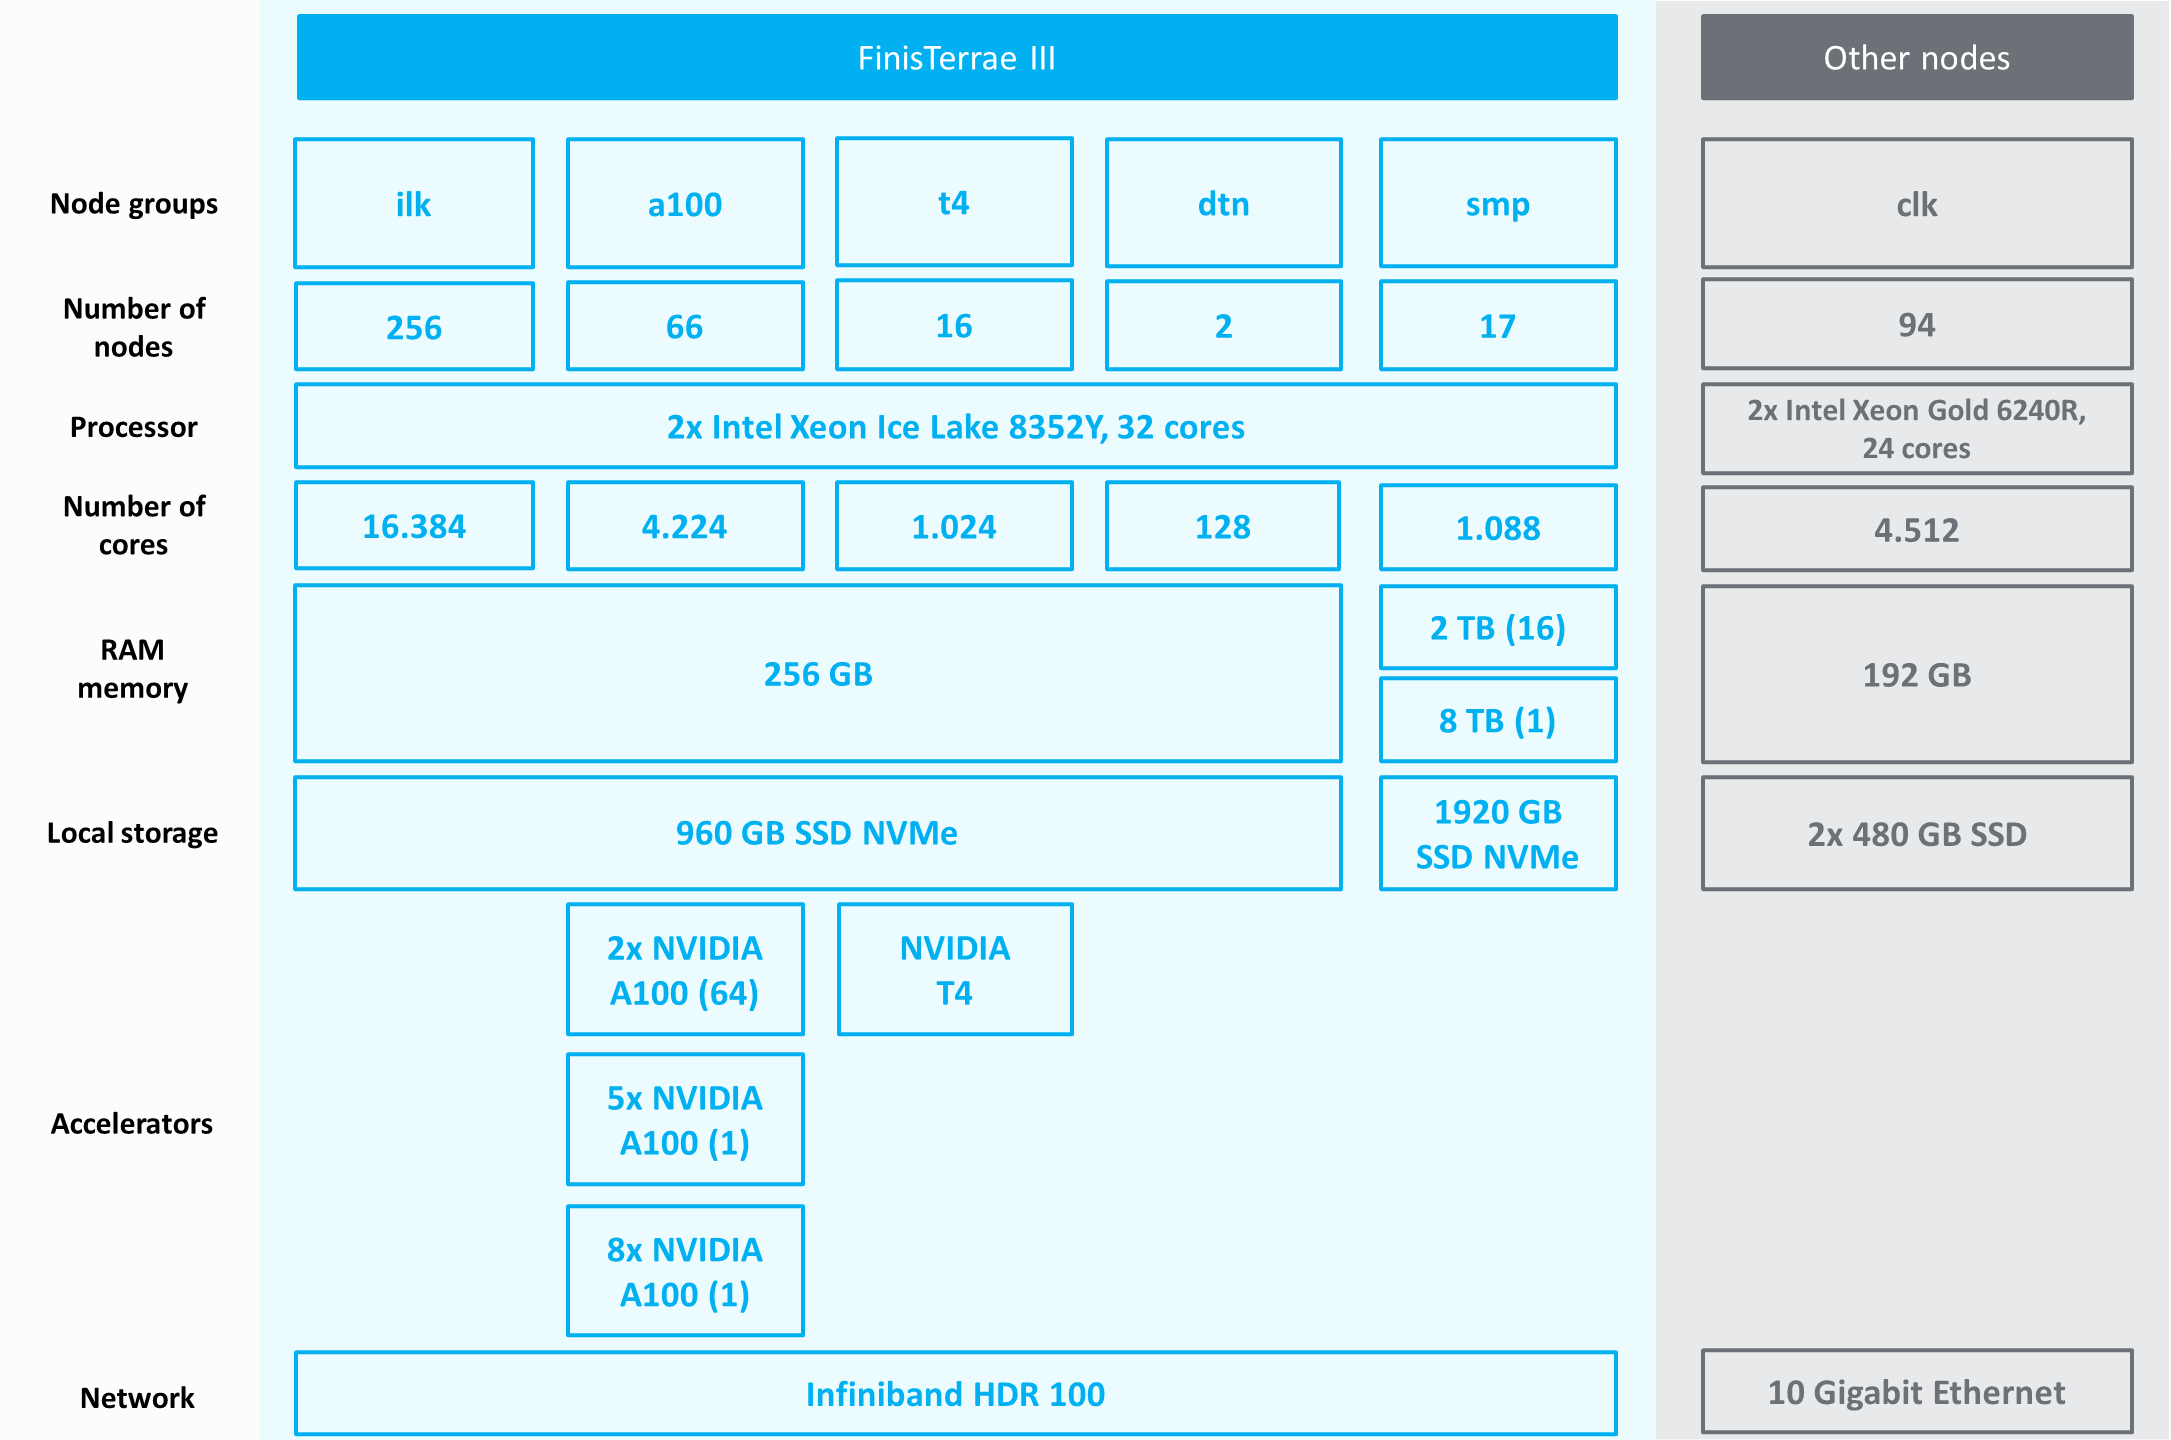
\includegraphics[width=\textwidth]{imaxes/FT3_schema}
    \caption{Esquema general de la arquitectura del supercomputador Finisterrae III}
    \label{fig:ft3-scheme}
\end{figure}

\subsection{Especificaciones técnicas de los nodos}\label{subsec:especificaciones-tecnicas-de-los-nodos}

La arquitectura del sistema se organiza en distintos tipos de nodos según el tipo de tarea a realizar tal y como se muestra en la figura~\ref{fig:ft3-scheme}.
Para este proyecto se han empleado cuatro clases de nodos:

\begin{itemize}
    \item \textbf{Nodos \texttt{ilk} (CPU)}: Diseñados para tareas de cómputo intensivo que no requieren aceleración por GPU. El Finisterrae III cuenta con 256 de estos nodos.
    Necesario para la versión cpu del proyecto.
    \item \textbf{Nodos \texttt{a100} (GPU)}: Equipados con unidades de procesamiento gráfico NVIDIA A100, orientados a cargas de trabajo en inteligencia artificial y procesamiento masivo de datos.
    Existen 64 nodos de este tipo.
    Necesario para simulaciones con hasta 2 GPUs.
    \item \textbf{Nodos \texttt{smp} (MEM)}: Similares a los nodos \texttt{ilk}, pero con una capacidad de memoria superior (2~TB), adecuados para trabajos que requieren un elevado uso de memoria.
    Necesario para la realización de pruebas de tamaño del árbol, tamaño de la base de datos y de resultados.
    \item \textbf{Nodo \texttt{a100-m8}}: Nodo especial para entrenamiento de modelos de IA y procesamiento multi-GPU, que dispone de 8 GPU NVIDIA A100 y mayor capacidad de memoria RAM.
    Necesario para la realización de simulaciones con más de 2 GPUs.
\end{itemize}

\subsection{Sistema de almacenamiento}\label{subsec:sistema-de-almacenamiento}

Además de los nodos de cómputo, el sistema cuenta con un almacenamiento en red de alta capacidad accesible desde todos los nodos.
Este almacenamiento está dividido en distintas áreas con cuotas y políticas específicas:

\begin{itemize}
    \item \textbf{\$HOME}: Espacio destinado a código fuente y programas. 
    Conectado mediante un enlace de baja velocidad, con límite de 10~GB o 100.000 archivos. 
    Incluye copias de seguridad diarias durante dos meses y \textit{snapshots} semanales.
    En el proyecto se utiliza para almacenar el código fuente, scripts y resultados de tests.
    \item \textbf{\$STORE}: Orientado al almacenamiento de resultados finales. 
    Límite de 500~GB o 300.000 archivos.
    Posee \textit{snapshots} durante tres días, sin copia de seguridad.
    Debido al poco espacio que ofrece, no es posible almacenar los resultados del proyecto en esta partición, por lo que no se utiliza.
    \item \textbf{\$LUSTRE}: Sistema de archivos de alta velocidad, destinado a la ejecución de simulaciones.
    No dispone de copias de seguridad ni \textit{snapshots}, y está limitado a 3~TB o 200.000 archivos.
    Gracias a su alta velocidad y la posibilidad de leer y escribir paralelamente archivos con gran eficiencia, se destina a almacenar y transformar los datos iniciales, así como almacenar los resultados finales.
\end{itemize}

\subsection{Modos de acceso}\label{subsec:modos-de-acceso}

El sistema ofrece cuatro modalidades principales de uso, en función del nivel de interactividad y la carga computacional requerida:

\begin{enumerate}
    \item \textbf{Uso interactivo}: acceso limitado y compartido mediante los nodos de \textit{login} (máximo 8~GB de memoria virtual).
    \item \textbf{Escritorios remotos}: acceso gráfico completo mediante X11; permite ejecutar aplicaciones con interfaz gráfica, aunque no es recomendable para simulaciones largas o que superen los 32~GB de memoria.
    \item \textbf{Nodos interactivos dedicados}: sesiones interactivas con recursos exclusivos mediante el comando \texttt{compute}, con un máximo de 64 núcleos y 247~GB de RAM durante 8 horas.
    \item \textbf{Sistema de colas}: uso mediante el gestor de colas \textbf{Slurm Workload Manager}~\cite{slurm}, indicado para simulaciones prolongadas o de gran escala.
    Los trabajos se envían mediante el comando \texttt{sbatch} (modo no interactivo) o \texttt{srun} (modo interactivo).
\end{enumerate}

En este proyecto se ha utilizado principalmente el sistema de colas de \textbf{Slurm} para las simulaciones, combinándolo con escritorios remotos para la ejecución de herramientas gráficas de análisis.
El acceso al sistema se realiza mediante SSH (\textit{Secure Shell}), utilizando el comando ssh user\_cesga@ft3.cesga.es.
El usuario es redirigido automáticamente a uno de los nodos de \textit{login}, desde los cuales se puede compilar software, preparar scripts o enviar trabajos al planificador.

\subsection{Módulos software}\label{subsec:modulos-software}
La gestión de aplicaciones en Finisterrae III se realiza mediante el sistema de módulos \textbf{Lmod}\footnote{Lmod: Environment Modules System. Disponible en: \url{https://lmod.readthedocs.io/}}, que permite cargar entornos modulares y establecer las variables de entorno correspondientes.
Dado el elevado número de dependencias entre aplicaciones y versiones, es necesario cargar un módulo jerárquico principal.
En este proyecto se ha utilizado el entorno base \texttt{cesga/2025}.

Los principales módulos empleados fueron:

\begin{itemize}
    \item \textbf{CMake}\footnote{CMake. Disponible en:\url{https://cmake.org/}}:
    Es una herramienta de automatización del proceso de compilación que permite generar de manera portable los archivos necesarios para construir proyectos en distintos sistemas y compiladores.
    En este caso facilita la gestión de dependencias, la compilación modular y la consistencia de pruebas locales y en la infraestructura HPC\@.

    \item \textbf{OpenMP}:
    Es una API que permite la programación paralela en sistemas de memoria compartida.
    Para una descripción detallada, véase la sección~\ref{subsec:openmp}.
    \item \textbf{CUDA}:
    Es una plataforma de computación paralela y un modelo de programación desarrollado por NVIDIA diseñado para aprovechar la potencia de sus GPUs con todo tipo de cálculos.
    Para una descripción detallada, véase la sección~\ref{subsec:cuda}.

    \item \textbf{Intel Compiler}:
    Es un conjunto de compiladores diseñados para obtener el máximo rendimiento en procesadores fabricados por Intel.
    Proporciona optimizaciones automáticas a nivel de vectorización, paralelización y uso eficiente de la memoria caché.

    \item \textbf{Intel VTune Profiler}\footnote{Intel VTune Profiler. Disponible en:\url{https://www.intel.com/content/www/us/en/developer/tools/vtune-profiler.html}}:
    Es una herramienta de análisis y perfilado de rendimiento desarrollada por Intel.
    Permite detectar cuellos de botella en el uso de CPU, memoria o E/S, ofreciendo métricas detalladas sobre la ejecución de los programas.
    Su integración con los compiladores Intel facilita la optimización iterativa del código y la evaluación del impacto de las mejoras implementadas.

    \item \textbf{NVIDIA HPC Compiler}:
    Forma parte del conjunto \textit{NVIDIA HPC SDK}, que incluye compiladores, bibliotecas y herramientas optimizadas para el desarrollo de aplicaciones de alto rendimiento en CPU y GPU.
    Especialmente diseñado para la compilación de aplicaciones CUDA de alto rendimiento.
    Además, proporcionan optimizaciones automáticas para GPU NVIDIA A100, como las presentes en el supercomputador Finisterrae III.

    \item \textbf{NVIDIA Nsight Compute}\footnote{Nvidia Nsight Compute. Disponible en:\url{https://developer.nvidia.com/nsight-compute}}:
    Es un analizador de rendimiento (\textit{profiler}) especializado para aplicaciones CUDA.
    Permite inspeccionar la ejecución de kernels en GPU, analizando métricas como la utilización de memoria global, el rendimiento de cada multiprocesador o el grado de ocupación de los núcleos CUDA.
    Es una herramienta fundamental para optimizar aplicaciones paralelas que utilizan GPU NVIDIA.

\end{itemize}

\section{Tecnologías de paralelización: OpenMP y CUDA}\label{sec:openmp-cuda}
En este proyecto se han empleado dos tecnologías principales para la paralelización del código: OpenMP, orientada a sistemas de memoria compartida, y CUDA, diseñada para aprovechar la capacidad de cómputo masivo de las GPU NVIDIA\@.

\subsection{OpenMP}\label{subsec:openmp}

\textbf{OpenMP}~\cite{openmp-spec} es una API de programación paralela en sistemas de memoria compartida.
Proporciona un conjunto de directivas que permiten transformar bucles y secciones de código secuenciales en regiones paralelas, sin necesidad de modificar la estructura principal del programa.
Su modelo de ejecución es del tipo \textit{fork–join}: el hilo principal crea un conjunto de hilos que ejecutan en paralelo una región determinada y, al finalizar, se sincronizan automáticamente.
El número de hilos se puede cambiar de forma dinámica utilizando la variable de entorno OMP\_NUM\_THREADS.
Esto permite adaptar el grado de paralelismo a los recursos disponibles del sistema sin recompilar el código.

La directiva más utilizada en nuestro código paralelo es \texttt{\#pragma omp parallel for}, que permite distribuir las iteraciones de un bucle entre varios hilos.
De esta forma, cada hilo ejecuta un subconjunto de iteraciones, reduciendo significativamente el tiempo total de ejecución en operaciones repetitivas sobre grandes volúmenes de datos.

\begin{lstlisting}[language=C,label={lst:lstlisting2}]
#pragma omp parallel for
for (int i = 0; i < N; i++) {
    array[i] = funcion(array[i]);
}
\end{lstlisting}

Esta directiva admite parámetros adicionales para controlar la distribución del trabajo, como \texttt{schedule(static)} o \texttt{schedule(dynamic)}, que determinan si las iteraciones se asignan de forma fija o adaptativa según la carga total y de cada hilo.

Cuando múltiples hilos contribuyen al cálculo de una misma variable acumulativa (por ejemplo, una suma, un máximo o una media), para evitar condiciones de carrera y sincronizaciones con alto coste, OpenMP ofrece la cláusula \texttt{reduction}, que crea una copia privada de la variable para cada hilo y combina los resultados al final de la región paralela.

\begin{lstlisting}[language=C,label={lst:lstlisting}]
double total = 0.0;
#pragma omp parallel for reduction(+:total)
for (int i = 0; i < N; i++) {
    total += valores[i];
}
\end{lstlisting}

Esto garantiza un resultado correcto y reproducible, sin necesidad de usar bloqueos o secciones críticas.

OpenMP incluye además mecanismos de sincronización dentro de una sección paralela:
\begin{itemize}
    \item \texttt{critical}: garantiza que una sección de código solo sea ejecutada por un hilo a la vez.
    \item \texttt{barrier}: obliga a que todos los hilos alcancen un punto antes de continuar.
    \item \texttt{atomic}: asegura que operaciones simples sobre variables compartidas se realicen de forma indivisible.
\end{itemize}

En general, el objetivo es minimizar el uso de sincronización para evitar bloqueos o esperas innecesarias.

\subsection{CUDA}\label{subsec:cuda}


\textbf{CUDA} (\textit{Compute Unified Device Architecture})~\cite{cuda-guide} es una plataforma de programación paralela desarrollada por NVIDIA que permite ejecutar código en las unidades de procesamiento gráfico (GPU).
A diferencia de OpenMP, que trabaja sobre arquitecturas de memoria compartida entre núcleos de CPU, CUDA explota el paralelismo masivo disponible en miles de núcleos de las GPU, ejecutando de forma simultánea un gran número de hilos.


En el modelo de programación CUDA, la GPU actúa como coprocesador y recibe el nombre de dispositivo.
El programa se inicia en la CPU, denominada host, que es responsable de decidir qué fragmento de código se ejecutará en la GPU, reservar la memoria necesaria y transferir los datos correspondientes.

A continuación, se crean múltiples hilos sobre los núcleos de la GPU, que trabajan en paralelo.
Cada hilo ejecuta el mismo código —denominado kernel— pero sobre datos distintos.
Los hilos se agrupan en bloques, dentro de los cuales pueden compartir memoria y sincronizarse entre sí.

Antes de lanzar el código CUDA, es necesario especificar el número de hilos por bloque y el número de bloques.
El número total de hilos será el producto de ambos valores.

Cada kernel se define con el calificador \texttt{\_\_global\_\_}, que indica que la función será ejecutada en el dispositivo pero invocada desde el host.
La llamada al kernel incluye la configuración de ejecución mediante los operadores \texttt{<<<...>>>}, que especifican el tamaño de la cuadrícula (\texttt{GRID\_SIZE}) y del bloque (\texttt{BLOCK\_SIZE}):




\begin{lstlisting}[language=C,label={lst:ejemplo_kernel}]
__global__ void compute(double *data, int N) {
    int i = blockIdx.x * blockDim.x + threadIdx.x;
    if (i < N) {
        data[i] = funcion(data[i]);
    }
}

// Lanzamiento del kernel
int BLOCK_SIZE = 256;
int GRID_SIZE  = (N + BLOCK_SIZE - 1) / BLOCK_SIZE;
compute<<<GRID_SIZE, BLOCK_SIZE>>>(d_data, N);
\end{lstlisting}

Cada hilo obtiene un identificador único combinando el índice del bloque (\texttt{blockIdx}) y el del hilo dentro del bloque (\texttt{threadIdx}).
Esta organización jerárquica permite distribuir grandes cantidades de datos de manera eficiente entre miles de hilos concurrentes.


La elección del tamaño de bloque (\texttt{BLOCK\_SIZE}) es un aspecto crítico para el rendimiento.
Valores demasiado pequeños infrautilizan la GPU, mientras que tamaños excesivos pueden provocar desbordamiento de registros o de memoria compartida.

El tamaño de la cuadrícula (\texttt{GRID\_SIZE}) se calcula de forma que todos los elementos de los datos sean procesados, incluso cuando el número total no sea múltiplo del tamaño de bloque:

\[
    \text{GRID\_SIZE} = \left\lceil \frac{N}{\text{BLOCK\_SIZE}} \right\rceil
\]

donde \(N\) es el número total de elementos a procesar.
En la práctica, tamaños de 128, 256 o 512 hilos por bloque suelen ofrecer un equilibrio adecuado entre ocupación y eficiencia, dependiendo de la arquitectura del dispositivo.

\subsubsection{Modelo de memoria}
El modelo de memoria de CUDA se organiza en varios niveles, cada uno con distinto alcance y velocidad:
\begin{itemize}
    \item \textbf{Memoria global}: accesible por todos los hilos y persistente durante la ejecución. Tiene gran capacidad, pero mayor latencia.
    \item \textbf{Memoria compartida}: compartida entre los hilos de un mismo bloque, de acceso rápido y útil para almacenar resultados intermedios.
    \item \textbf{Registros y memoria local}: privados para cada hilo, con acceso muy rápido.
\end{itemize}

La GPU no comparte el mismo espacio de direcciones que la CPU, por lo que es necesario realizar transferencias explícitas de datos entre el host y el dispositivo.
Estas operaciones se realizan mediante funciones como:

\begin{lstlisting}[language=C,label={lst:ejemplo_copia}]
cudaMalloc((void**)&d_data, N * sizeof(double)); // Reserva en GPU
cudaMemcpy(d_data, h_data, N * sizeof(double), cudaMemcpyHostToDevice);  // Copia al dispositivo
cudaMemcpy(h_data, d_data, N * sizeof(double), cudaMemcpyDeviceToHost);  // Copia al host
cudaFree(d_data);  // Liberación de memoria en GPU
\end{lstlisting}

Lo habitual es mantener los datos en GPU todo lo posible durante varias etapas de cálculo, ya que el traspaso a CPU es muy costoso.

\subsubsection{Ejecución asíncrona y \textit{streams}}
CUDA permite solapar la transferencia de datos con la ejecución de kernels mediante el uso de \textit{streams}.
Un \textit{stream} es una cola de operaciones que se ejecutan de forma secuencial, pero diferentes \textit{streams} pueden operar en paralelo si los recursos del dispositivo lo permiten.
Esto permite aprovechar mejor la concurrencia entre cómputo y comunicación:

\begin{lstlisting}[language=C,label={lst:ejemplo_asincrono}]
cudaStream_t stream;
cudaStreamCreate(&stream);
cudaMemcpyAsync(d_data, h_data, N * sizeof(double), cudaMemcpyHostToDevice, stream);
compute<<<GRID_SIZE, BLOCK_SIZE, 0, stream>>>(d_data, N);
cudaMemcpyAsync(h_data, d_data, N * sizeof(double), cudaMemcpyDeviceToHost, stream);
cudaStreamSynchronize(stream);
cudaStreamDestroy(stream);
\end{lstlisting}

El uso de \texttt{cudaMemcpyAsync()} en combinación con \texttt{streams} permite realizar copias asíncronas, reduciendo el tiempo de espera y mejorando la utilización global del dispositivo.

\subsubsection{Gestión de múltiples GPU}
En sistemas con más de una GPU, CUDA permite seleccionar el dispositivo sobre el que se ejecutará cada parte del código mediante la función \texttt{cudaSetDevice()}.
Esto resulta esencial para distribuir la carga de trabajo y aprovechar los recursos de forma equilibrada.

\begin{lstlisting}[language=C,label={lst:ejemplo_setdevice}]
int deviceCount;
cudaGetDeviceCount(&deviceCount);
for (int dev = 0; dev < deviceCount; dev++) {
    cudaSetDevice(dev);
    compute<<<GRID_SIZE, BLOCK_SIZE>>>(d_data[dev], N_local);
}
\end{lstlisting}

Cada GPU mantiene su propio espacio de memoria y contexto de ejecución, por lo que las transferencias entre dispositivos deben realizarse mediante \texttt{cudaMemcpyPeer()} si está disponible la comunicación directa entre ellos.

\subsubsection{Sincronización y control de ejecución}
CUDA incluye diversas funciones de sincronización para garantizar la coherencia en los cálculos:
\begin{itemize}
    \item \texttt{\_\_syncthreads()}: sincroniza todos los hilos dentro de un bloque.
    \item \texttt{cudaDeviceSynchronize()}: bloquea el host hasta que todas las operaciones pendientes en la GPU hayan finalizado.
    \item \texttt{cudaStreamSynchronize(stream)}: espera a que finalicen las operaciones de un \textit{stream} concreto.
\end{itemize}

El uso correcto de estas funciones permite evitar conflictos de acceso a memoria compartida y asegurar el orden adecuado de las operaciones.



